\documentclass[a4paper,12pt,oneside,openany]{report}	
\usepackage{url}

\usepackage{layout}
\setlength{\textwidth}{15.0 cm}
\setlength{\textheight}{25.0 cm}


\usepackage[english,brazil]{babel}
\usepackage{pagina}	% pagina-padrao
\usepackage{indentfirst}		% for indent
\usepackage[utf8x]{inputenc}
\usepackage{graphics,epsfig}
\usepackage{graphics}
\graphicspath{{./figuras/}}
\usepackage{pstricks,pst-node,pst-tree}
\usepackage{alltt}
%\usepackage{makeidx}
%\makeindex
\usepackage[figuresright]{rotating} % for saydways tables and figures
\usepackage{enumerate}			% for configuration of enumerate environment
\usepackage{amsmath}
\usepackage{amssymb}
\usepackage{multirow}

\setcounter{secnumdepth}{3}	% numeracao ate subsubsecao
\setcounter{tocdepth}{2}	% indice ate subsubsecao

\usepackage{longtable}


\begin{document}


\begin{center}
\textbf{UNIVERSIDADE FEDERAL DO RIO DE JANEIRO}
\vspace{-0.2cm}

\textbf{ESCOLA POLITÉCNICA}
\vspace{-0.2cm}

\textbf{DEPARTAMENTO DE ENGENHARIA ELETRÔNICA E DE COMPUTAÇÃO}
\vspace{0.8cm}

\underline{\textbf{PROPOSTA DE PROJETO DE GRADUAÇÃO}}

Aluno: Pedro Henrique Barbosa Nori
\vspace{-0.2cm}

pedrobnori@poli.ufrj.br

Orientador:
\end{center}

\textbf{1. TÍTULO}

	Técnicas de Aprendizado de Máquina Aplicadas ao Mercado de Ações

\vspace{0.4cm}
\textbf{2. ÊNFASE}

Computação

\vspace{0.4cm}
\textbf{3. TEMA}

O tema deste trabalho visa a aplicação de inteligência artificial às negociações do mercado financeiro. Nesse sentido, o problema a ser analisado é a identificação de tendências de alta na variação dos preços das ações, bem como a análise de risco para entrada e saída em operações de um determinado ativo.

\vspace{0.4cm}
\textbf{4. DELIMITAÇÃO}

O objeto de estudo do trabalho se restringe aos dados reais negociados na Bolsa de Valores de São Paulo (BM\&FBovespa), disponibilizados gratuitamente pela instituição. A janela temporal é diária devido as dificuldades de armazenamento de dados para janeras menores. Portanto, toda a análise será voltada para tomada de decisões de Swing Trade, isto é, operações de compra e venda de ações numa janela de tempo maior que um dia.

\vspace{0.4cm}
\textbf{5. JUSTIFICATIVA}

O número de investidores na Bolsa de Valores brasileira tem apresentado um crescimento cada vez 
maior \cite{historicopf}. 
Mesmo após a crise decorrida pela pandemia COVID-19, os números continuam crescentes

\vspace{0.4cm}
\textbf{6. OBJETIVO}

O objetivo geral deste trabalho é implementar um software livre que permita processar um banco de dados de modo a torná-lo dessensibilizado, podendo assim ser utilizado para apoiar atividades de desenvolvimento de sistemas sem a preocupação com vazamento de dados por parte de terceiros.

Sendo assim, os objetivos específicos a serem atingidos na implementação são: (1) O software deve remover informações que permitam associar indivíduos a um conjunto de dados; (2) O software deve substituir dados reais sensíveis por dados gerados a partir de estatísticas; (3) O software não deve alterar a estrutura do modelo de dados existente, somente o seu conteúdo.;

\vspace{0.4cm}
\textbf{7. METODOLOGIA}

Este trabalho inicialmente consiste num estudo das técnicas de anonimização de dados anteriormente aplicadas em dados médicos, que possuem necessidade de cuidados especiais de privacidade anterior a existência das leis de proteção de dados gerais, com o intuito de verificar como e quais técnicas podem ser utilizadas fora do contexto da informática para medicina. Para esta etapa inicial será feita uma revisão da literatura do assunto.

Em seguida, serão analisadas soluções de software livre existentes para verificar a implementação das técnicas exploradas anteriormente. Esta etapa contemplará softwares cuja licença seja aberta e estejam disponíveis no Github, tendo por objetivo caracterizar as funcionalidades existentes de modo a definir os requisitos do software a ser implementado, de maneira que este traga vantagens em relação as soluções existentes.

A partir da definição dos requisitos na etapa anterior, tem-se por inicio o desenvolvimento do código-fonte da nova solução. Esta solução será implementada utilizando a linguagem de programação Python, por se tratar de uma linguagem aberta e possuir suporte multiplataforma. Também será utilizada a biblioteca SQLAlchemy para implementar as atividades de acesso e manipulação dos bancos de dados, pois esta biblioteca fornece uma camada de abstração sobre diferentes implementações de APIs SQL\cite{sqlalch}, possibilitando que o projeto possa ser utilizado com diferentes implementações de bancos de dados SQL.

O alvo final deste trabalho é completar a implementação de um Minimum Viable Product com as funcionalidades determinadas anteriormente a ser validado sobre bases de dados públicas disponíveis na internet.

\vspace{0.4cm}
\textbf{8. MATERIAIS}
	
Serão utilizados software livres para estudo. Linguagem Python. Plataforma Github para controle de versão do código-fonte.

\vspace{0.4cm}
\textbf{9. CRONOGRAMA}

Apresentada graficamente conforme a Figura \ref{Fig:Cronograma}.

Fase 1: Estudo inicial sobre impacto socioeconômico causado pela visão de dados como commoditie

Fase 2: Análise bibliográfica de técnicas de privacidade e tópicos afins.

Fase 3: Estudo e levantamento das características de softwares de anonimização de código-aberto.

Fase 4: Implementação do código-fonte.

Fase 5: Testes com bases de dados públicas.

Fase 6: Revisão da Monografia

Fase 7: Elaboração da monografia


\begin{figure}
\begin{center}
\parbox[h]{14cm}
  {
  \begin{center}
  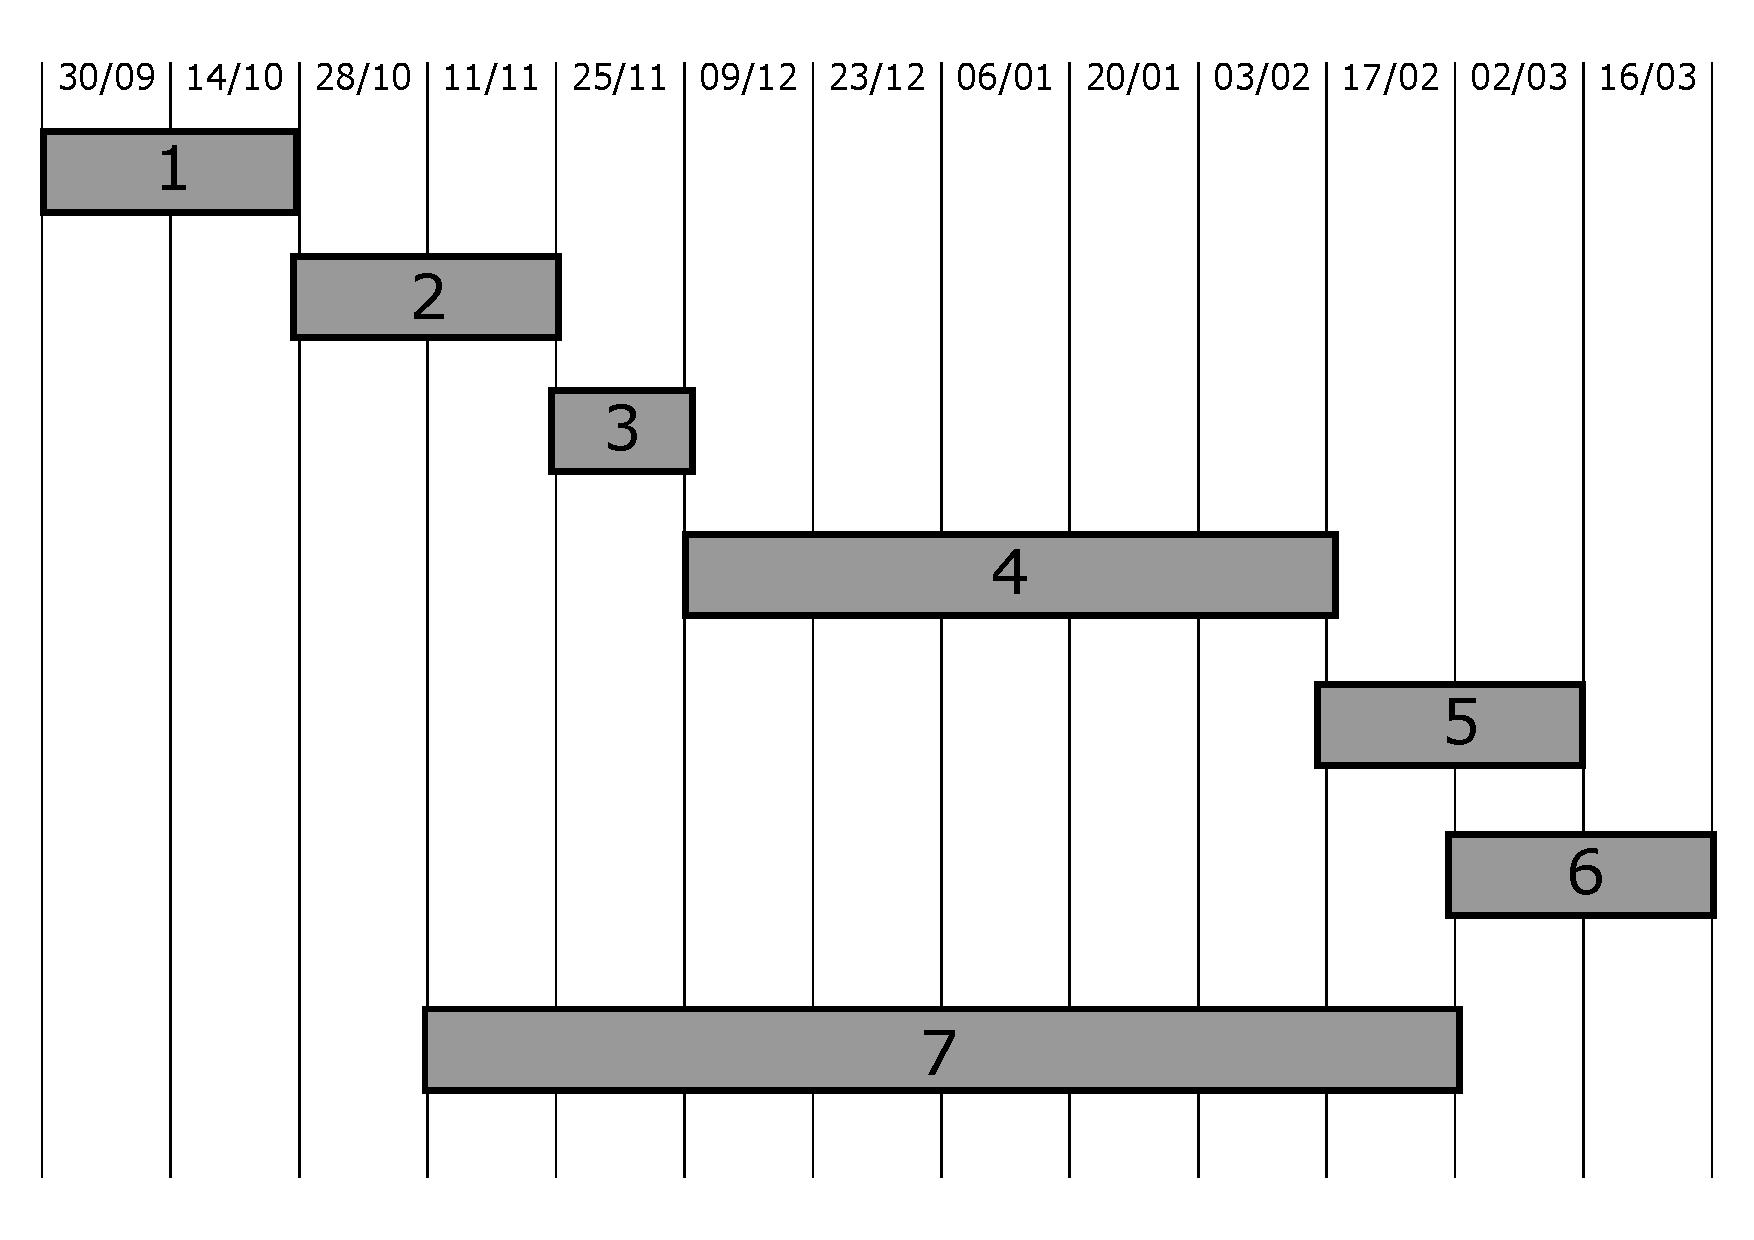
\includegraphics[scale=0.45]{Figuras/gantt.pdf}
  \caption[\small{\textit{Planejamento}}]{\label{Fig:Cronograma} \footnotesize{\textit{Planejamento}}}
  \end{center}
  }
\end{center}
\end{figure} 

\begin{thebibliography}{}

\bibitem{historicopf}
Histórico de Pessoas Físicas, 
\url{http://www.b3.com.br/pt\_br/market-data-e-indices/servicos-de-dados/market-data/consultas/mercado-a-vista/historico-pessoas-fisicas/}, 2020 (Acessado em Junho/2020)

\bibitem{investidores-covid} BATISTA, Henrique G. 
"Bolsa ganha mais de 300 mil investidores na pandemia e ultrapassa 2 milhões de ‘CPFs’", 
\\\texttt{https://oglobo.globo.com/economia/bolsa-ganha-mais-de-300-mil-investidores-na-pandemia-ultrapassa-2-milhoes-de-cpfs-24434447}, 2020 (Acessado em junho/2020)

\end{thebibliography}

      \vspace{2cm}
      \noindent
Rio de Janeiro, 14 de junho de 2020

      \vspace{0.5cm}
      \begin{flushright}
         \parbox{10cm}{
            \hrulefill

            \vspace{-.375cm}
            \centering{Pedro Henrique Barbosa Nori - Aluno}

            \vspace{0.9cm}
            \hrulefill

            \vspace{-.375cm}
            \centering{ - Orientador}
 
            \vspace{0.9cm}
         }
      \end{flushright}
      \vfill
      
\end{document}
